% Design schematic of the XSuM-MicroBooNE surrogate (proposed, 2026-11-18; nothing of it is implemented yet).
% Same layout as XSuM-MINERvA's paper/schematic/model_schematic.tex so the two can be read side by side.
% Compile: bash docs/technote/build.sh.
\documentclass[tikz,border=6pt]{standalone}
\usetikzlibrary{positioning,fit,arrows.meta,calc,backgrounds}
\usepackage[T1]{fontenc}
\usepackage{amsmath,amssymb}
\usepackage{helvet}\renewcommand{\familydefault}{\sfdefault}
\definecolor{ink}{HTML}{222222}
\definecolor{cin}{HTML}{0072B2}    % inputs
\definecolor{csame}{HTML}{009E73}  % ported from XSuM-MINERvA unchanged
\definecolor{cnew}{HTML}{E69F00}   % new for MicroBooNE
\definecolor{cwait}{HTML}{8C8C8C}  % waits on the hit-level curation
\definecolor{cout}{HTML}{555555}
\tikzset{
  box/.style={draw=ink, line width=1.2pt, rounded corners=3pt, fill=white, align=left, inner sep=6pt, font=\small, text=ink},
  head/.style={box, text width=126mm},
  same/.style={draw=csame, fill=csame!6},
  new/.style={draw=cnew, fill=cnew!8},
  wait/.style={draw=cwait, dashed, fill=white},
  stage/.style={font=\footnotesize\bfseries, text=ink!80, anchor=south west},
  dim/.style={font=\scriptsize, text=ink!70},
  arr/.style={-{Latex[length=2.2mm]}, line width=0.7pt, draw=ink},
  arrd/.style={arr, dashed},
  arrc/.style={arr, dotted, line width=0.9pt},
}
\begin{document}
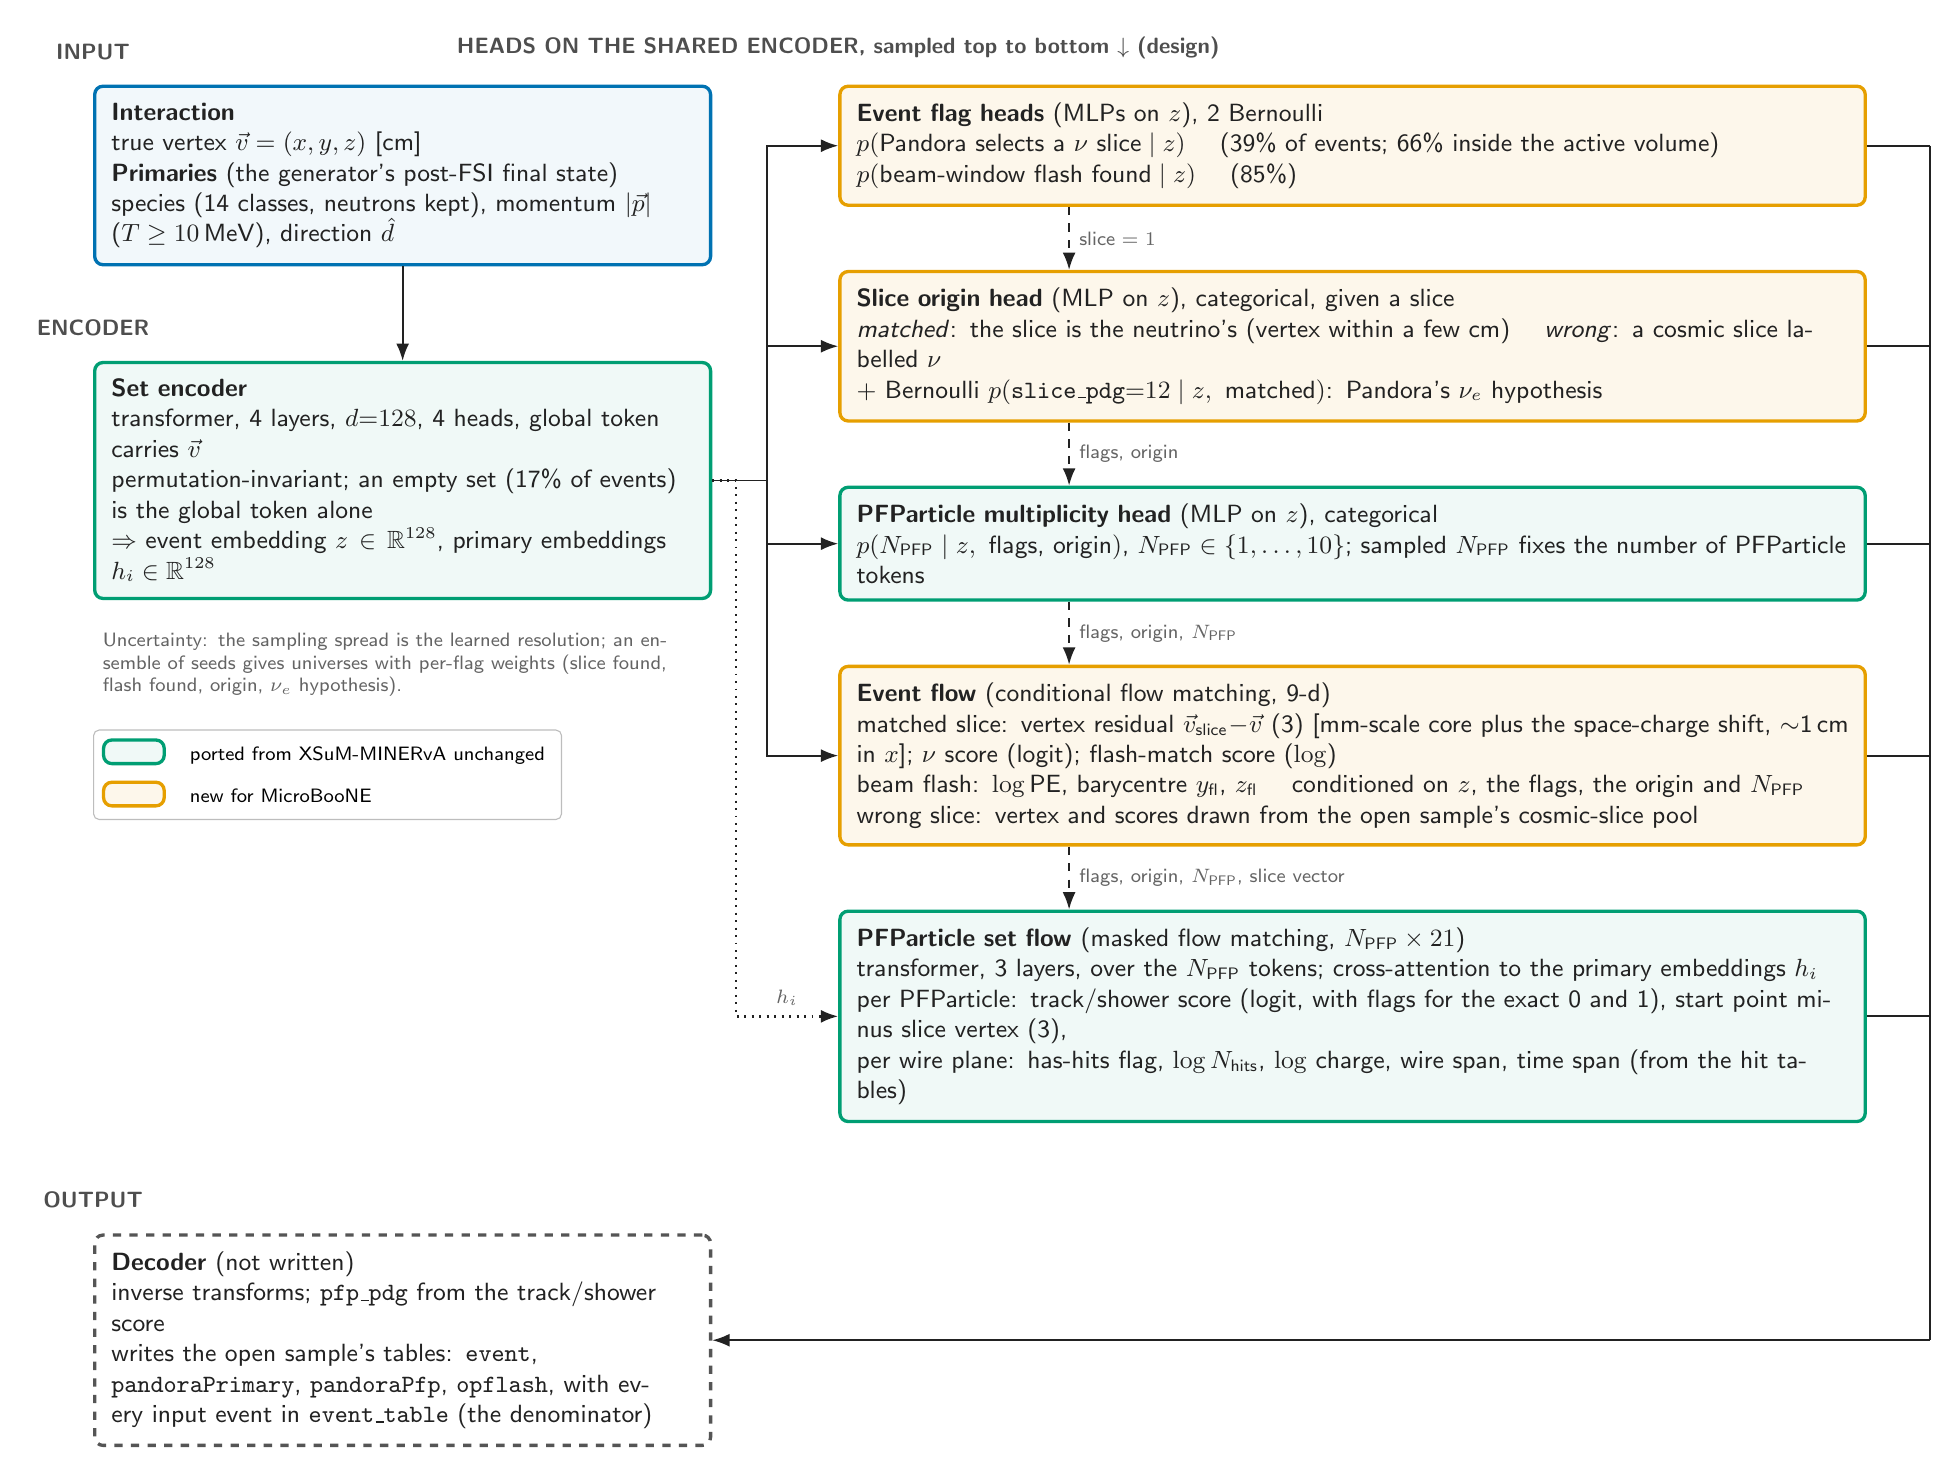
\begin{tikzpicture}[node distance=7mm and 9mm]

% ---------------- inputs and encoder (left column) ----------------
\node[box, draw=cin, fill=cin!5, text width=74mm] (gen) {\textbf{Interaction}\\
  true vertex $\vec v=(x,y,z)$ [cm]\\
  \textbf{Primaries} (the generator's post-FSI final state)\\
  species (14 classes, neutrons kept), momentum $|\vec p|$ ($T\ge 10$\,MeV), direction $\hat d$};
\node[box, same, text width=74mm, below=12mm of gen.south west, anchor=north west] (enc) {\textbf{Set encoder}\\
  transformer, 4 layers, $d{=}128$, 4 heads, global token carries $\vec v$\\
  permutation-invariant; an empty set (17\% of events) is the global token alone\\
  $\Rightarrow$ event embedding $z\in\mathbb{R}^{128}$, primary embeddings $h_i\in\mathbb{R}^{128}$};

% ---------------- heads (right column) ----------------
\node[head, new, right=16mm of gen.north east, anchor=north west] (flag) {\textbf{Event flag heads} (MLPs on $z$), 2 Bernoulli\\
  $p(\text{Pandora selects a $\nu$ slice}\mid z)$ \quad (39\% of events; 66\% inside the active volume)\\
  $p(\text{beam-window flash found}\mid z)$ \quad (85\%)};
\node[head, new, below=8mm of flag.south west, anchor=north west] (orig) {\textbf{Slice origin head} (MLP on $z$), categorical, given a slice\\
  \emph{matched}: the slice is the neutrino's (vertex within a few cm) \quad \emph{wrong}: a cosmic slice labelled $\nu$\\
  + Bernoulli $p(\texttt{slice\_pdg}{=}12\mid z,\ \text{matched})$: Pandora's $\nu_e$ hypothesis};
\node[head, same, below=8mm of orig.south west, anchor=north west] (card) {\textbf{PFParticle multiplicity head} (MLP on $z$), categorical\\
  $p(N_\text{PFP}\mid z,\ \text{flags, origin})$, $N_\text{PFP}\in\{1,\dots,10\}$; sampled $N_\text{PFP}$ fixes the number of PFParticle tokens};
\node[head, new, below=8mm of card.south west, anchor=north west] (ev) {\textbf{Event flow} (conditional flow matching, 9-d)\\
  matched slice: vertex residual $\vec v_\text{slice}-\vec v$ (3) [mm-scale core plus the space-charge shift, $\sim$1\,cm in $x$]; $\nu$ score (logit); flash-match score ($\log$)\\
  beam flash: $\log\text{PE}$, barycentre $y_\text{fl}$, $z_\text{fl}$ \quad conditioned on $z$, the flags, the origin and $N_\text{PFP}$\\
  wrong slice: vertex and scores drawn from the open sample's cosmic-slice pool};
\node[head, same, below=8mm of ev.south west, anchor=north west] (pf) {\textbf{PFParticle set flow} (masked flow matching, $N_\text{PFP}\times 21$)\\
  transformer, 3 layers, over the $N_\text{PFP}$ tokens; cross-attention to the primary embeddings $h_i$\\
  per PFParticle: track/shower score (logit, with flags for the exact 0 and 1), start point minus slice vertex (3),\\
  per wire plane: has-hits flag, $\log N_\text{hits}$, $\log$ charge, wire span, time span (from the hit tables)};

% ---------------- decoder ----------------
\node[box, draw=cout, dashed, text width=74mm, anchor=north west] (dec) at ($(enc.south west |- pf.south)+(0,-14mm)$) {\textbf{Decoder} (not written)\\
  inverse transforms; \texttt{pfp\_pdg} from the track/shower score\\
  writes the open sample's tables: \texttt{event}, \texttt{pandoraPrimary}, \texttt{pandoraPfp}, \texttt{opflash}, with every input event in \texttt{event\_table} (the denominator)};

% ---------------- arrows ----------------
\draw[arr] (gen.south) -- (enc.north);
\coordinate (fan) at ($(enc.east)+(7mm,0)$);
\foreach \h in {flag,orig,card,ev} { \draw[arr] (enc.east) -- (fan) |- (\h.west); }
\draw[arrc] (enc.east) -- ++(3mm,0) |- (pf.west) node[dim, pos=0.75, above] {$h_i$};
\draw[arrd] ([xshift=-36mm]flag.south) -- ([xshift=-36mm]orig.north) node[dim, pos=0.5, right] {slice${}=1$};
\draw[arrd] ([xshift=-36mm]orig.south) -- ([xshift=-36mm]card.north) node[dim, pos=0.5, right] {flags, origin};
\draw[arrd] ([xshift=-36mm]card.south) -- ([xshift=-36mm]ev.north) node[dim, pos=0.5, right] {flags, origin, $N_\text{PFP}$};
\draw[arrd] ([xshift=-36mm]ev.south) -- ([xshift=-36mm]pf.north) node[dim, pos=0.5, right] {flags, origin, $N_\text{PFP}$, slice vector};
\coordinate (bus) at ($(flag.east)+(8mm,0)$);
\foreach \h in {flag,orig,card,ev,pf} { \draw[line width=0.7pt, draw=ink] (\h.east) -- (\h.east -| bus); }
\draw[line width=0.7pt, draw=ink] (flag.east -| bus) -- (bus |- dec.east);
\draw[arr] (bus |- dec.east) -- (dec.east);

% ---------------- labels and legend ----------------
\node[stage, above=2mm of gen.north west] {INPUT};
\node[stage, above=2mm of enc.north west] {ENCODER};
\node[stage, above=2mm of flag.north west] {HEADS ON THE SHARED ENCODER, sampled top to bottom $\downarrow$ (design)};
\node[stage, above=2mm of dec.north west] {OUTPUT};
\node[dim, text width=74mm, align=left, below=3mm of enc.south west, anchor=north west] (unc) {Uncertainty: the sampling spread is the learned resolution; an ensemble of seeds gives universes with per-flag weights (slice found, flash found, origin, $\nu_e$ hypothesis).};
\matrix[draw=ink!30, rounded corners=2pt, fill=white, inner sep=3pt, column sep=2mm, row sep=1mm, font=\scriptsize, below=3mm of unc.south west, anchor=north west] {
  \node[box, same, text width=7mm, minimum height=3mm, inner sep=1pt]{}; & \node{ported from XSuM-MINERvA unchanged}; \\
  \node[box, new, text width=7mm, minimum height=3mm, inner sep=1pt]{}; & \node{new for MicroBooNE}; \\
};
\end{tikzpicture}
\end{document}
